% Options for packages loaded elsewhere
\PassOptionsToPackage{unicode}{hyperref}
\PassOptionsToPackage{hyphens}{url}
%
\documentclass[
]{article}
\usepackage{lmodern}
\usepackage{amssymb,amsmath}
\usepackage{ifxetex,ifluatex}
\ifnum 0\ifxetex 1\fi\ifluatex 1\fi=0 % if pdftex
  \usepackage[T1]{fontenc}
  \usepackage[utf8]{inputenc}
  \usepackage{textcomp} % provide euro and other symbols
\else % if luatex or xetex
  \usepackage{unicode-math}
  \defaultfontfeatures{Scale=MatchLowercase}
  \defaultfontfeatures[\rmfamily]{Ligatures=TeX,Scale=1}
\fi
% Use upquote if available, for straight quotes in verbatim environments
\IfFileExists{upquote.sty}{\usepackage{upquote}}{}
\IfFileExists{microtype.sty}{% use microtype if available
  \usepackage[]{microtype}
  \UseMicrotypeSet[protrusion]{basicmath} % disable protrusion for tt fonts
}{}
\makeatletter
\@ifundefined{KOMAClassName}{% if non-KOMA class
  \IfFileExists{parskip.sty}{%
    \usepackage{parskip}
  }{% else
    \setlength{\parindent}{0pt}
    \setlength{\parskip}{6pt plus 2pt minus 1pt}}
}{% if KOMA class
  \KOMAoptions{parskip=half}}
\makeatother
\usepackage{xcolor}
\IfFileExists{xurl.sty}{\usepackage{xurl}}{} % add URL line breaks if available
\IfFileExists{bookmark.sty}{\usepackage{bookmark}}{\usepackage{hyperref}}
\hypersetup{
  pdftitle={Ej.1 Representación Gráfica en R},
  pdfauthor={Ramon Ceballos},
  hidelinks,
  pdfcreator={LaTeX via pandoc}}
\urlstyle{same} % disable monospaced font for URLs
\usepackage[margin=1in]{geometry}
\usepackage{color}
\usepackage{fancyvrb}
\newcommand{\VerbBar}{|}
\newcommand{\VERB}{\Verb[commandchars=\\\{\}]}
\DefineVerbatimEnvironment{Highlighting}{Verbatim}{commandchars=\\\{\}}
% Add ',fontsize=\small' for more characters per line
\usepackage{framed}
\definecolor{shadecolor}{RGB}{248,248,248}
\newenvironment{Shaded}{\begin{snugshade}}{\end{snugshade}}
\newcommand{\AlertTok}[1]{\textcolor[rgb]{0.94,0.16,0.16}{#1}}
\newcommand{\AnnotationTok}[1]{\textcolor[rgb]{0.56,0.35,0.01}{\textbf{\textit{#1}}}}
\newcommand{\AttributeTok}[1]{\textcolor[rgb]{0.77,0.63,0.00}{#1}}
\newcommand{\BaseNTok}[1]{\textcolor[rgb]{0.00,0.00,0.81}{#1}}
\newcommand{\BuiltInTok}[1]{#1}
\newcommand{\CharTok}[1]{\textcolor[rgb]{0.31,0.60,0.02}{#1}}
\newcommand{\CommentTok}[1]{\textcolor[rgb]{0.56,0.35,0.01}{\textit{#1}}}
\newcommand{\CommentVarTok}[1]{\textcolor[rgb]{0.56,0.35,0.01}{\textbf{\textit{#1}}}}
\newcommand{\ConstantTok}[1]{\textcolor[rgb]{0.00,0.00,0.00}{#1}}
\newcommand{\ControlFlowTok}[1]{\textcolor[rgb]{0.13,0.29,0.53}{\textbf{#1}}}
\newcommand{\DataTypeTok}[1]{\textcolor[rgb]{0.13,0.29,0.53}{#1}}
\newcommand{\DecValTok}[1]{\textcolor[rgb]{0.00,0.00,0.81}{#1}}
\newcommand{\DocumentationTok}[1]{\textcolor[rgb]{0.56,0.35,0.01}{\textbf{\textit{#1}}}}
\newcommand{\ErrorTok}[1]{\textcolor[rgb]{0.64,0.00,0.00}{\textbf{#1}}}
\newcommand{\ExtensionTok}[1]{#1}
\newcommand{\FloatTok}[1]{\textcolor[rgb]{0.00,0.00,0.81}{#1}}
\newcommand{\FunctionTok}[1]{\textcolor[rgb]{0.00,0.00,0.00}{#1}}
\newcommand{\ImportTok}[1]{#1}
\newcommand{\InformationTok}[1]{\textcolor[rgb]{0.56,0.35,0.01}{\textbf{\textit{#1}}}}
\newcommand{\KeywordTok}[1]{\textcolor[rgb]{0.13,0.29,0.53}{\textbf{#1}}}
\newcommand{\NormalTok}[1]{#1}
\newcommand{\OperatorTok}[1]{\textcolor[rgb]{0.81,0.36,0.00}{\textbf{#1}}}
\newcommand{\OtherTok}[1]{\textcolor[rgb]{0.56,0.35,0.01}{#1}}
\newcommand{\PreprocessorTok}[1]{\textcolor[rgb]{0.56,0.35,0.01}{\textit{#1}}}
\newcommand{\RegionMarkerTok}[1]{#1}
\newcommand{\SpecialCharTok}[1]{\textcolor[rgb]{0.00,0.00,0.00}{#1}}
\newcommand{\SpecialStringTok}[1]{\textcolor[rgb]{0.31,0.60,0.02}{#1}}
\newcommand{\StringTok}[1]{\textcolor[rgb]{0.31,0.60,0.02}{#1}}
\newcommand{\VariableTok}[1]{\textcolor[rgb]{0.00,0.00,0.00}{#1}}
\newcommand{\VerbatimStringTok}[1]{\textcolor[rgb]{0.31,0.60,0.02}{#1}}
\newcommand{\WarningTok}[1]{\textcolor[rgb]{0.56,0.35,0.01}{\textbf{\textit{#1}}}}
\usepackage{graphicx,grffile}
\makeatletter
\def\maxwidth{\ifdim\Gin@nat@width>\linewidth\linewidth\else\Gin@nat@width\fi}
\def\maxheight{\ifdim\Gin@nat@height>\textheight\textheight\else\Gin@nat@height\fi}
\makeatother
% Scale images if necessary, so that they will not overflow the page
% margins by default, and it is still possible to overwrite the defaults
% using explicit options in \includegraphics[width, height, ...]{}
\setkeys{Gin}{width=\maxwidth,height=\maxheight,keepaspectratio}
% Set default figure placement to htbp
\makeatletter
\def\fps@figure{htbp}
\makeatother
\setlength{\emergencystretch}{3em} % prevent overfull lines
\providecommand{\tightlist}{%
  \setlength{\itemsep}{0pt}\setlength{\parskip}{0pt}}
\setcounter{secnumdepth}{-\maxdimen} % remove section numbering

\title{Ej.1 Representación Gráfica en R}
\author{Ramon Ceballos}
\date{19/1/2021}

\begin{document}
\maketitle

\hypertarget{ejercicios}{%
\section{Ejercicios}\label{ejercicios}}

\begin{enumerate}
\def\labelenumi{\arabic{enumi}.}
\tightlist
\item
  Con una sola instrucción, dibujad el gráfico de la función
  y=x\^{}2−3x+30 entre −15 y 15. De título, poned ``Una parábola''. De
  etiquetas, en el eje 0X poned, en formato matemático, ``x''; y en el
  eje 0Y, introducid y=x\^{}2−3x+30, también en formato matemático.
  Tenéis que utilizar la función curve().
\end{enumerate}

\begin{Shaded}
\begin{Highlighting}[]
\KeywordTok{curve}\NormalTok{(x}\OperatorTok{^}\DecValTok{2-3}\OperatorTok{*}\NormalTok{x}\OperatorTok{+}\DecValTok{30}\NormalTok{,}\OperatorTok{-}\DecValTok{15}\NormalTok{,}\DecValTok{15}\NormalTok{, }
      \DataTypeTok{main =} \StringTok{"Una parábola"}\NormalTok{, }
      \DataTypeTok{xlab =} \KeywordTok{expression}\NormalTok{(x), }
      \DataTypeTok{ylab =} \KeywordTok{expression}\NormalTok{(}\DataTypeTok{y=}\NormalTok{x}\OperatorTok{^}\DecValTok{2-3}\OperatorTok{*}\NormalTok{x}\OperatorTok{+}\DecValTok{3}\NormalTok{))}
\end{Highlighting}
\end{Shaded}

\begin{center}\includegraphics{1-Representación-Grafica-en-R_files/figure-latex/unnamed-chunk-1-1} \end{center}

\begin{enumerate}
\def\labelenumi{\arabic{enumi}.}
\setcounter{enumi}{1}
\tightlist
\item
  Considerando lo que habéis obtenido en el ejercicio anterior y siendo
  y = f(x) = x\^{}2−3x+30 e I = {[}-15:15{]}, si en vez de utilizar la
  función curve(), utilizamos la función plot(), ¿es correcta la
  sentencia plot(f(I)) para representar la curva f en el intervalo I? En
  otras palabras, dan ambas sentencias la misma gráfica? Obviamente, en
  la sentencia plot(f(I)) se han omitido el resto de parámetros
  requeridos en el ejercicio anterior porque no influyen para nada en la
  curva. Tanto si la respuesta es afirmativa como negativa, cread la
  función f en R y argumentad vuestra respuesta, considerando todos los
  parámetros requeridos (título y etiquetas de ambos ejes).
\end{enumerate}

\begin{Shaded}
\begin{Highlighting}[]
\NormalTok{f =}\StringTok{ }\ControlFlowTok{function}\NormalTok{ (x)\{x}\OperatorTok{^}\DecValTok{2-3}\OperatorTok{*}\NormalTok{x}\OperatorTok{+}\DecValTok{30}\NormalTok{\}}
\NormalTok{sec =}\StringTok{ }\KeywordTok{c}\NormalTok{(}\OperatorTok{-}\DecValTok{15}\OperatorTok{:}\DecValTok{15}\NormalTok{)}

\KeywordTok{plot}\NormalTok{(sec,}\KeywordTok{f}\NormalTok{(sec), }
     \DataTypeTok{type =}\StringTok{"l"}\NormalTok{,}
     \DataTypeTok{main =} \StringTok{"Una parábola"}\NormalTok{,}
     \DataTypeTok{xlab =} \KeywordTok{expression}\NormalTok{(x),}
     \DataTypeTok{ylab =} \KeywordTok{expression}\NormalTok{(}\DataTypeTok{y=}\NormalTok{x}\OperatorTok{^}\DecValTok{2-3}\OperatorTok{*}\NormalTok{x}\OperatorTok{+}\DecValTok{3}\NormalTok{))}
\end{Highlighting}
\end{Shaded}

\begin{center}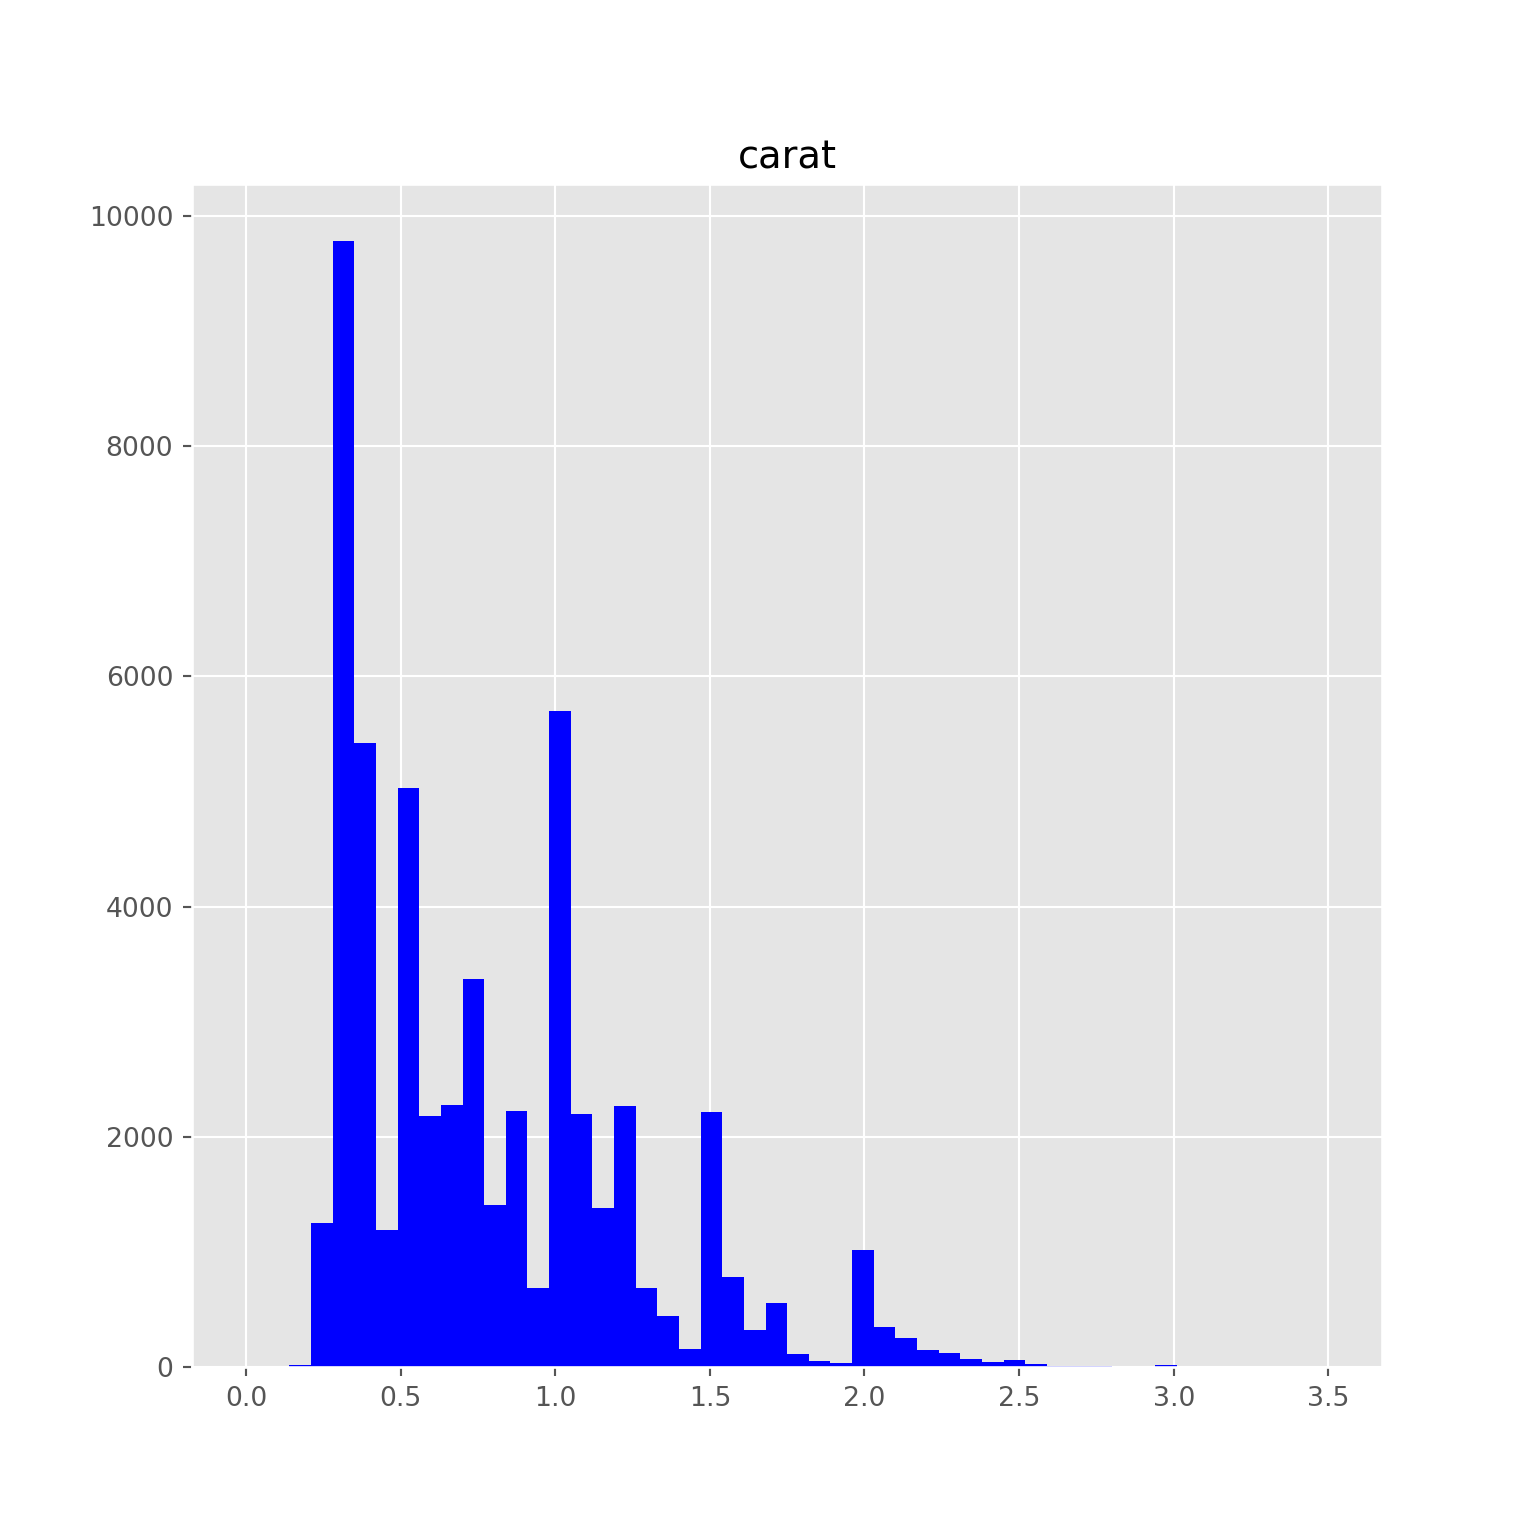
\includegraphics{1-Representación-Grafica-en-R_files/figure-latex/unnamed-chunk-2-1} \end{center}

\begin{enumerate}
\def\labelenumi{\arabic{enumi}.}
\setcounter{enumi}{2}
\tightlist
\item
  Dibuja un gráfico semilogarítmico de la función y = 5x2\^{}x entre -10
  y 25. Utilizad la función curve(). Mostrad solo la etiqueta del eje
  0Y, que ponga ``y = 5x2\^{}x'' en formato matemático.
\end{enumerate}

\begin{Shaded}
\begin{Highlighting}[]
\KeywordTok{curve}\NormalTok{(}\DecValTok{5}\OperatorTok{*}\DecValTok{2}\OperatorTok{^}\NormalTok{x,}\OperatorTok{-}\DecValTok{10}\NormalTok{,}\DecValTok{25}\NormalTok{, }
      \DataTypeTok{ylab =} \KeywordTok{expression}\NormalTok{(}\DataTypeTok{y =} \DecValTok{5}\NormalTok{(}\DecValTok{2}\OperatorTok{^}\NormalTok{x)),}
      \DataTypeTok{xlab =} \StringTok{""}\NormalTok{,}
      \DataTypeTok{log =} \StringTok{"y"}\NormalTok{)}
\end{Highlighting}
\end{Shaded}

\begin{center}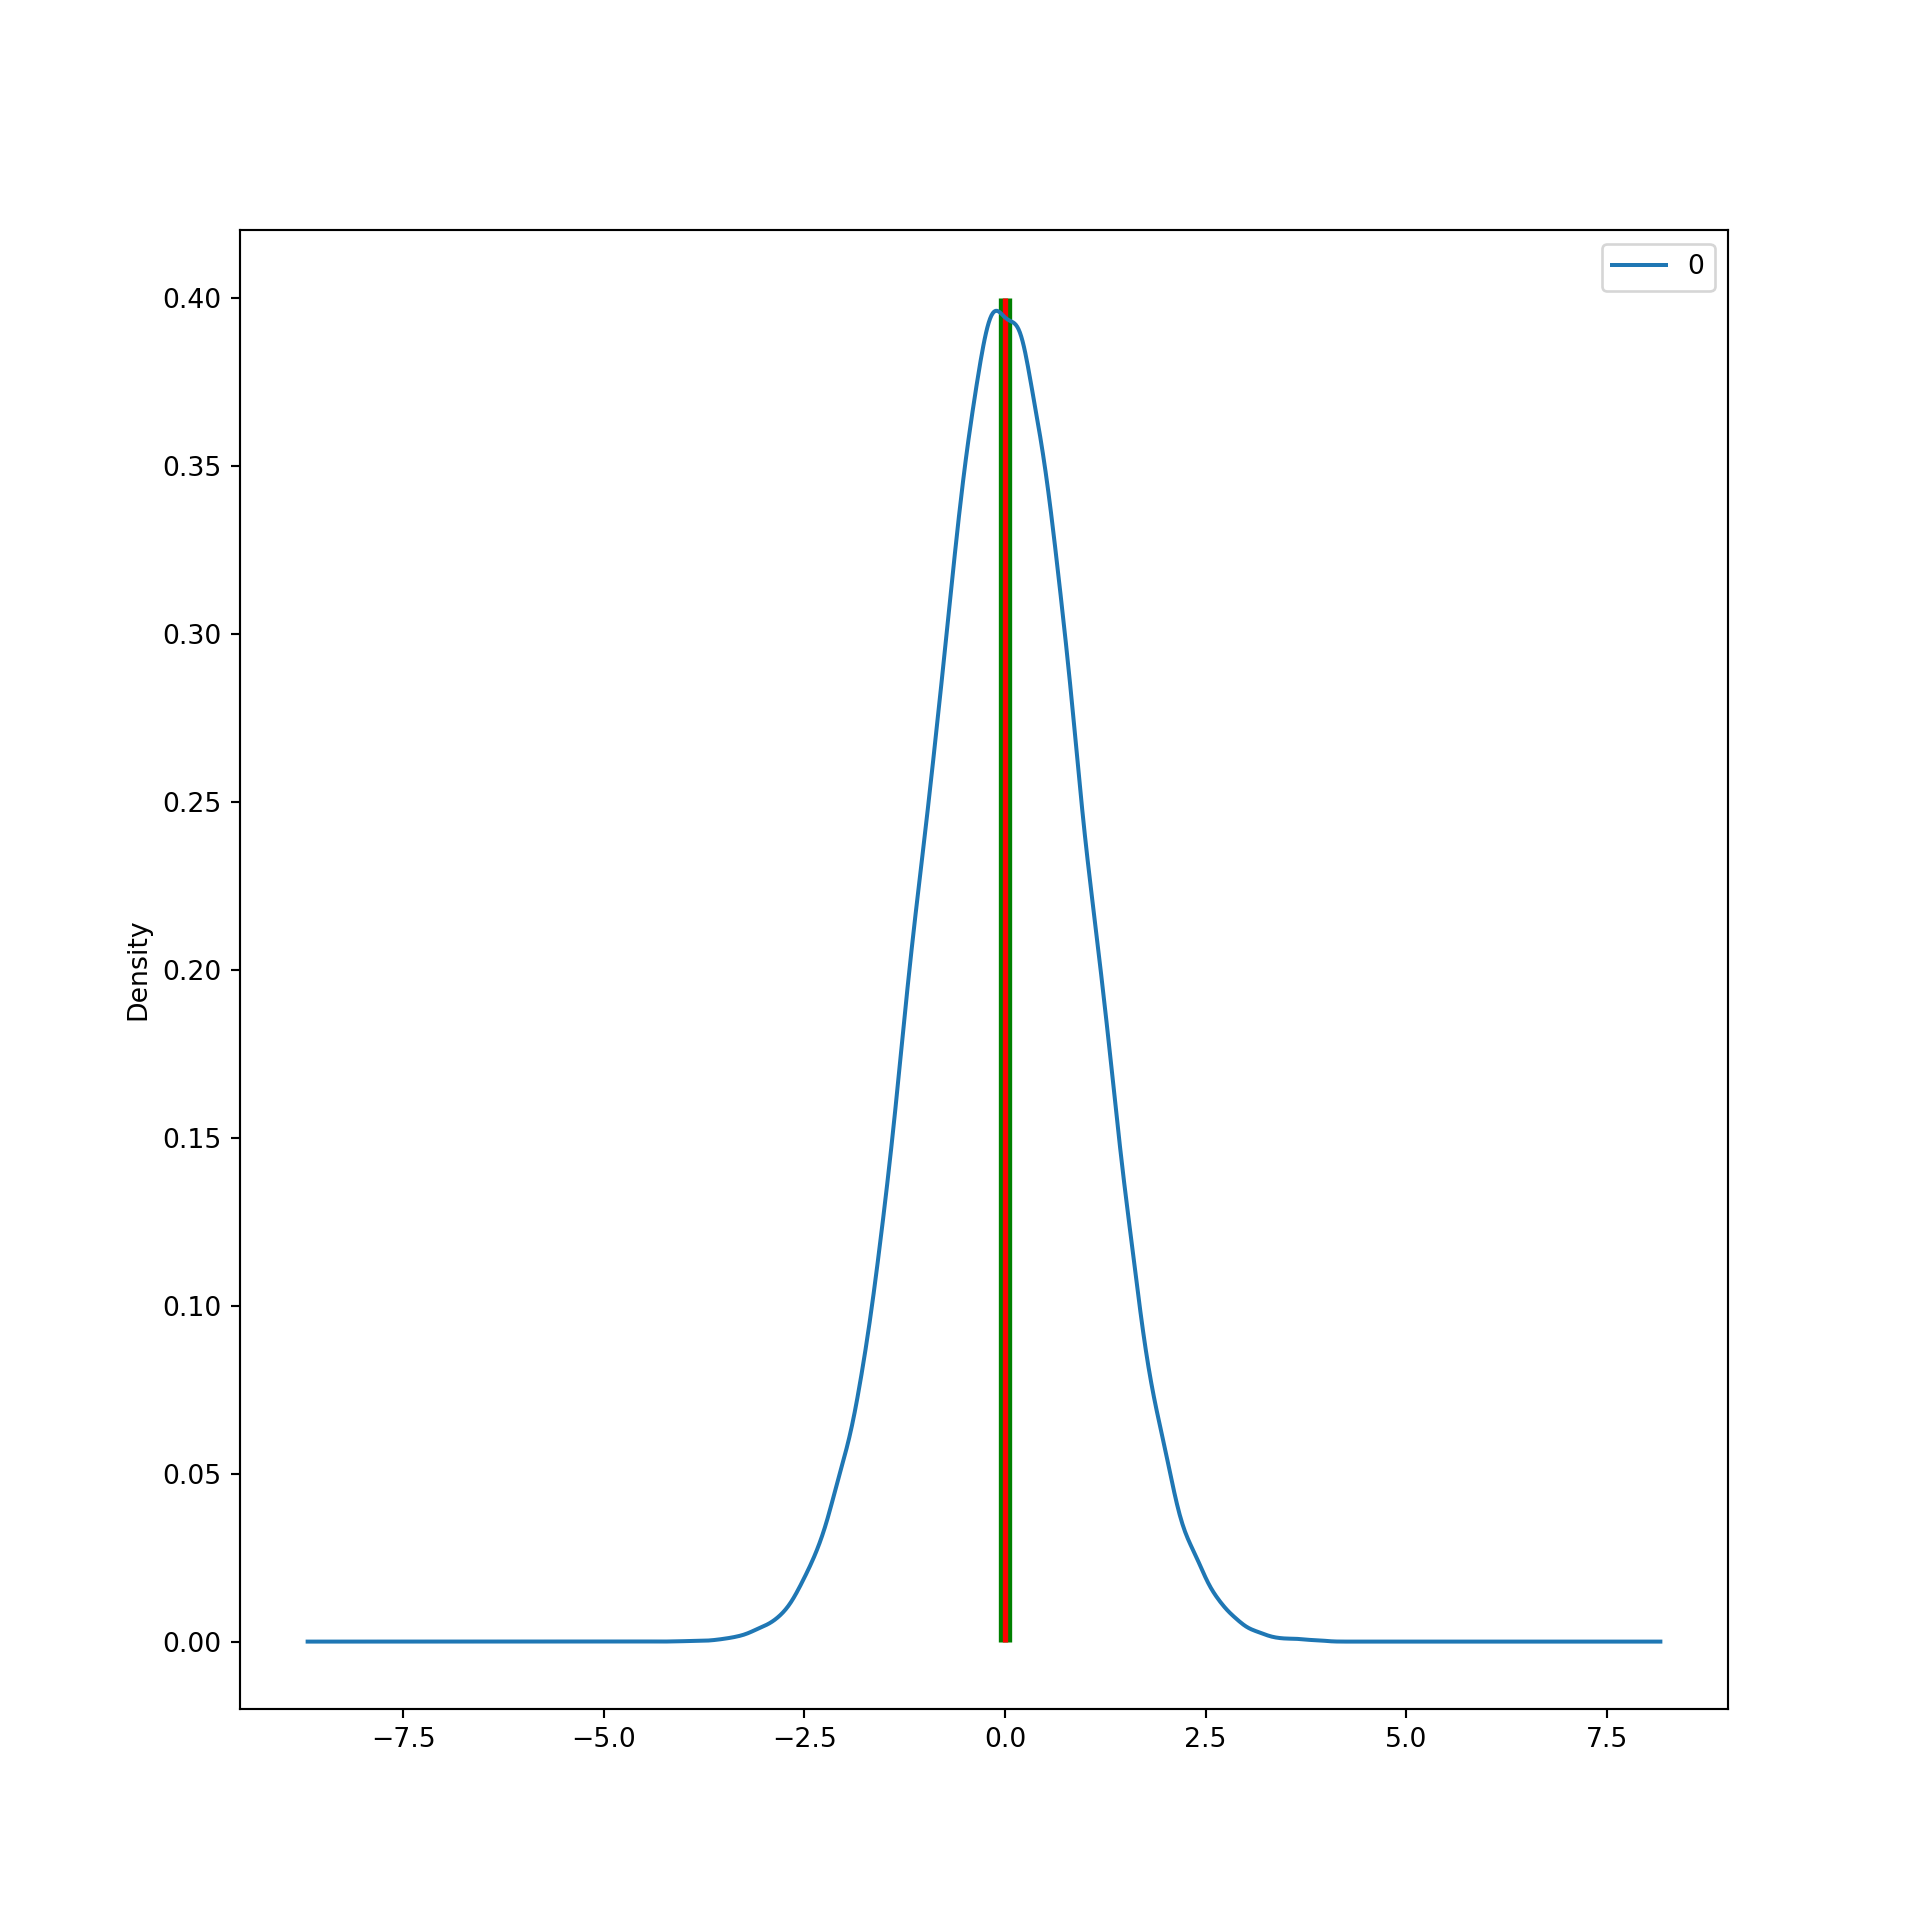
\includegraphics{1-Representación-Grafica-en-R_files/figure-latex/unnamed-chunk-3-1} \end{center}

\begin{enumerate}
\def\labelenumi{\arabic{enumi}.}
\setcounter{enumi}{3}
\tightlist
\item
  Dibuja el gráfico de la función y\_1 = 3x utilizando la función
  curve(). Añade la curva y\_2=-3x, entre -10 y 20. El gráfico no debe
  mostrar ninguna etiqueta. La primera curva debe ser de color azul y la
  segunda, de color verde. Ponedle de título ``2 rectas'' y de subtítulo
  ``Dos rectas con pendiente opuesto''. Añadid al gráfico un recuadro
  (con la esquina superior izquierda en el punto (13,10)) que indique
  que la función 3x es la azul y la -3x verde.
\end{enumerate}

\begin{Shaded}
\begin{Highlighting}[]
\KeywordTok{curve}\NormalTok{(}\DecValTok{3}\OperatorTok{*}\NormalTok{x,}\OperatorTok{-}\DecValTok{10}\NormalTok{,}\DecValTok{20}\NormalTok{, }\DataTypeTok{col =} \StringTok{"blue"}\NormalTok{,}
      \DataTypeTok{ylab =}\StringTok{""}\NormalTok{, }\DataTypeTok{xlab =} \StringTok{""}\NormalTok{,}
      \DataTypeTok{main =} \StringTok{"2 rectas"}\NormalTok{, }
      \DataTypeTok{sub =} \StringTok{"Dos rectas con pendiente opuesta"}\NormalTok{,}
      \DataTypeTok{ylim =}\KeywordTok{c}\NormalTok{(}\OperatorTok{-}\DecValTok{60}\NormalTok{,}\DecValTok{60}\NormalTok{),}
      \DataTypeTok{xlim =} \KeywordTok{c}\NormalTok{(}\OperatorTok{-}\DecValTok{10}\NormalTok{,}\DecValTok{20}\NormalTok{))}

\KeywordTok{curve}\NormalTok{(}\OperatorTok{-}\DecValTok{3}\OperatorTok{*}\NormalTok{x,}\OperatorTok{-}\DecValTok{10}\NormalTok{,}\DecValTok{20}\NormalTok{, }\DataTypeTok{col =}\StringTok{"green"}\NormalTok{,}
      \DataTypeTok{add =} \OtherTok{TRUE}\NormalTok{)}

\KeywordTok{legend}\NormalTok{(}\DataTypeTok{x=}\DecValTok{13}\NormalTok{,}\DataTypeTok{y=}\DecValTok{10}\NormalTok{,}
       \DataTypeTok{legend =} \KeywordTok{c}\NormalTok{(}\KeywordTok{expression}\NormalTok{(}\DecValTok{3}\OperatorTok{*}\NormalTok{x),}\KeywordTok{expression}\NormalTok{(}\OperatorTok{-}\DecValTok{3}\OperatorTok{*}\NormalTok{x)),}
       \DataTypeTok{col =} \KeywordTok{c}\NormalTok{(}\StringTok{"blue"}\NormalTok{,}\StringTok{"green"}\NormalTok{),}
       \DataTypeTok{lty =} \DecValTok{1}\NormalTok{)}
\end{Highlighting}
\end{Shaded}

\begin{center}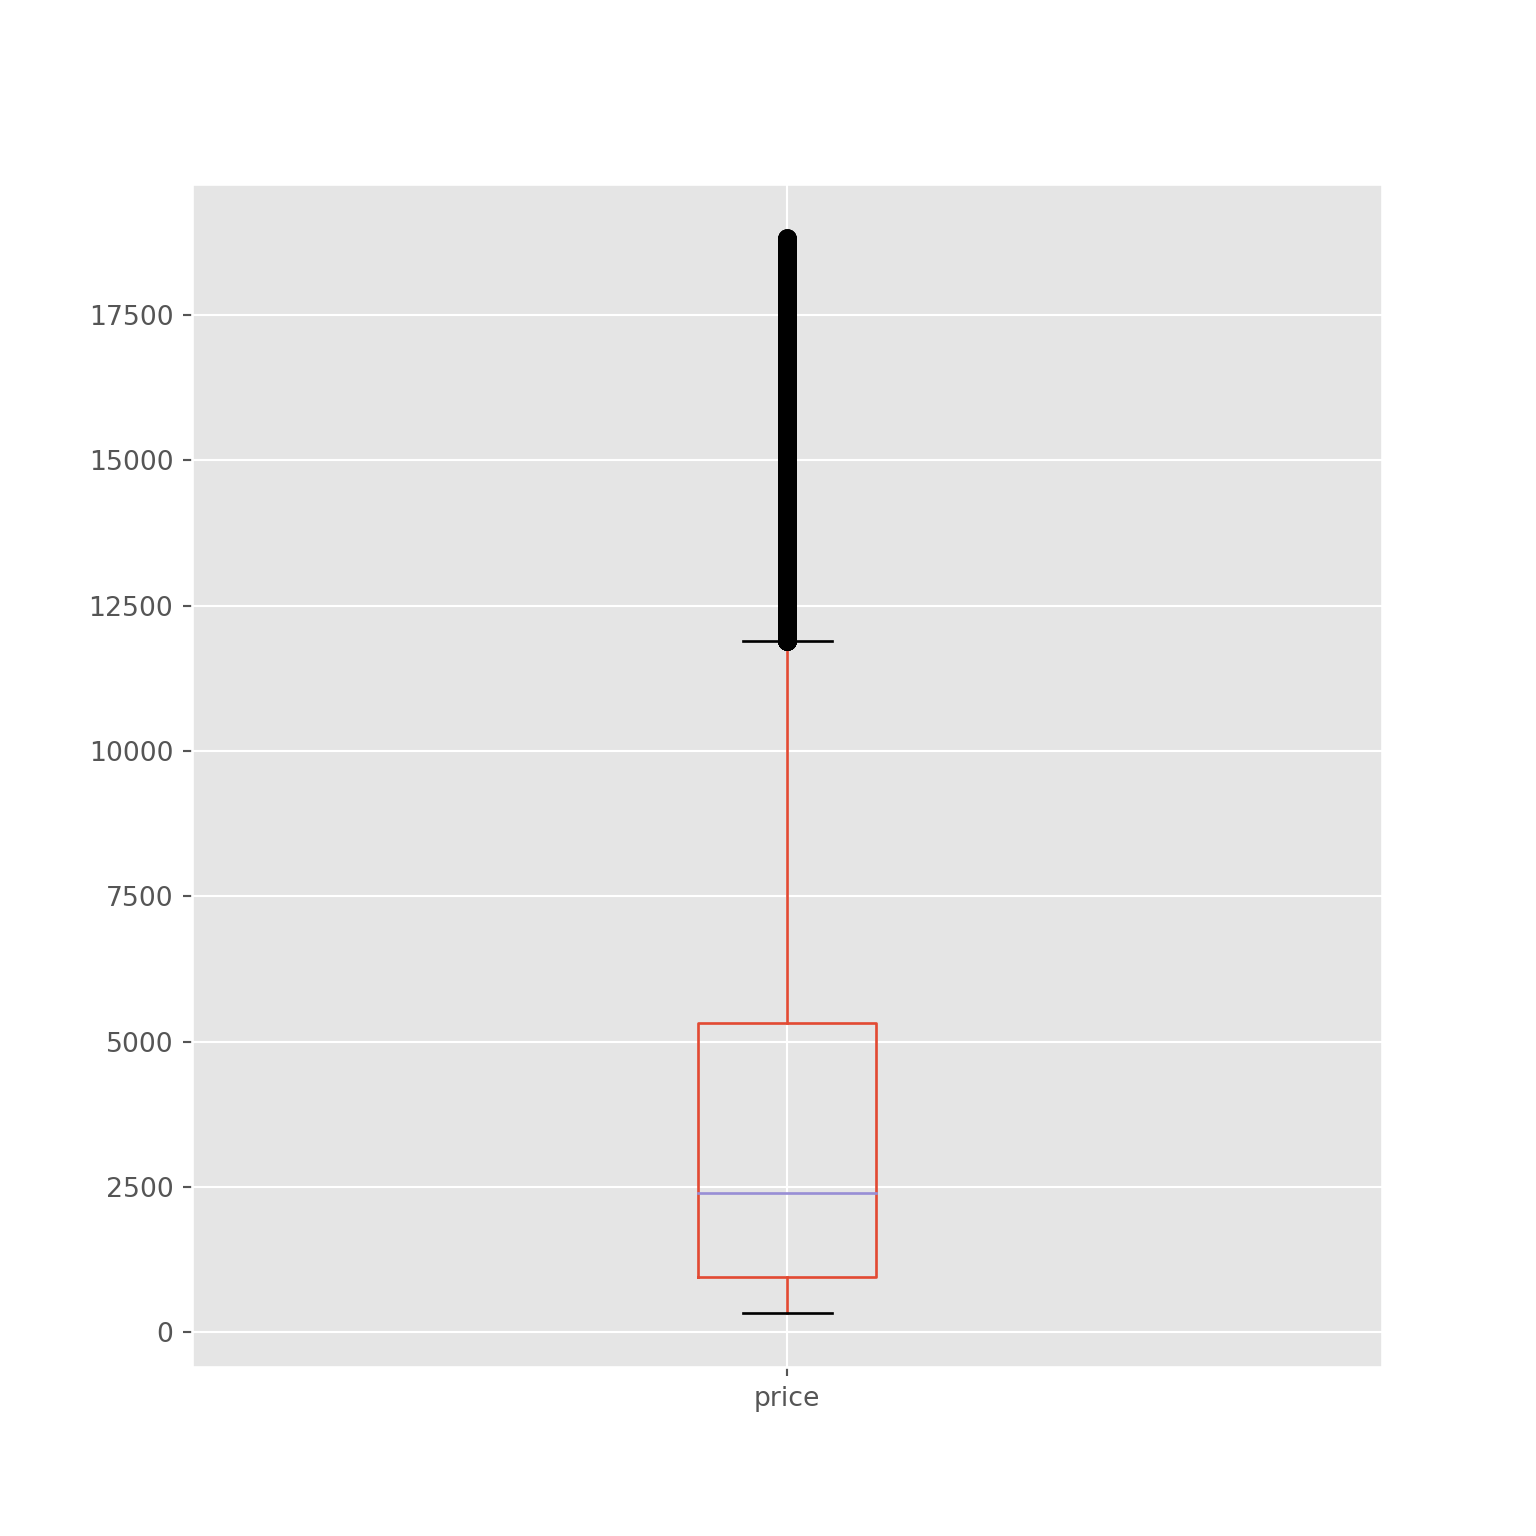
\includegraphics{1-Representación-Grafica-en-R_files/figure-latex/unnamed-chunk-4-1} \end{center}

\begin{enumerate}
\def\labelenumi{\arabic{enumi}.}
\setcounter{enumi}{4}
\tightlist
\item
  Dad la instrucción que añada a un gráfico anterior la recta horizontal
  y = 0 de color rojo con un grosor de 5 puntos.
\end{enumerate}

\begin{Shaded}
\begin{Highlighting}[]
\KeywordTok{curve}\NormalTok{(}\DecValTok{3}\OperatorTok{*}\NormalTok{x,}\OperatorTok{-}\DecValTok{10}\NormalTok{,}\DecValTok{20}\NormalTok{, }\DataTypeTok{col =} \StringTok{"blue"}\NormalTok{)}

\KeywordTok{abline}\NormalTok{(}\DataTypeTok{h=}\DecValTok{0}\NormalTok{, }\DataTypeTok{col =} \StringTok{"red"}\NormalTok{,}
       \DataTypeTok{lwd =} \DecValTok{5}\NormalTok{)}
\end{Highlighting}
\end{Shaded}

\begin{center}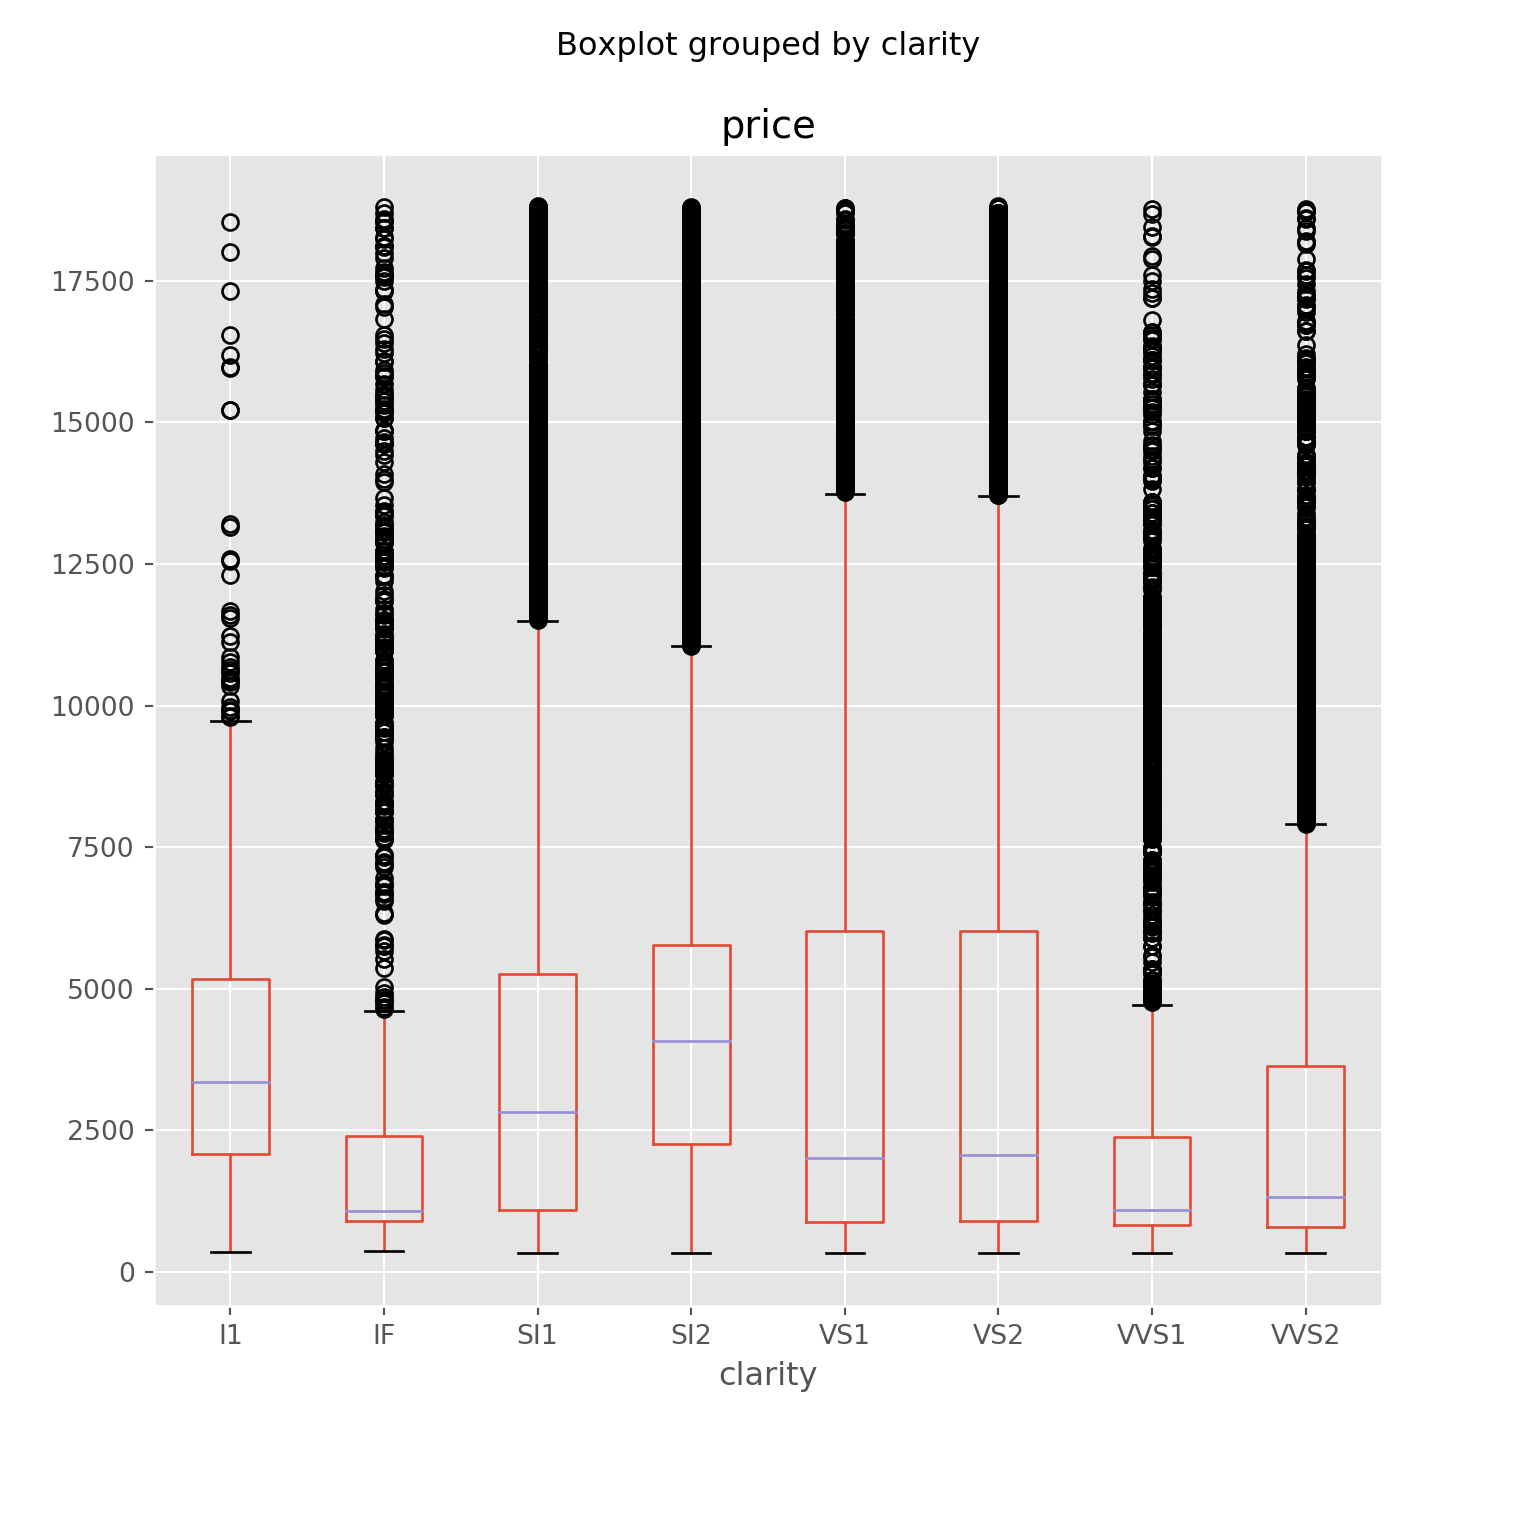
\includegraphics{1-Representación-Grafica-en-R_files/figure-latex/unnamed-chunk-5-1} \end{center}

\begin{enumerate}
\def\labelenumi{\arabic{enumi}.}
\setcounter{enumi}{5}
\tightlist
\item
  Dad la instrucción que añada a un gráfico anterior la recta y = 2x+7
  de color azul con un grosor de 2 puntos.
\end{enumerate}

\begin{Shaded}
\begin{Highlighting}[]
\KeywordTok{curve}\NormalTok{(}\DecValTok{3}\OperatorTok{*}\NormalTok{x,}\OperatorTok{-}\DecValTok{10}\NormalTok{,}\DecValTok{20}\NormalTok{, }\DataTypeTok{col =} \StringTok{"brown"}\NormalTok{)}

\KeywordTok{curve}\NormalTok{(}\DecValTok{2}\OperatorTok{*}\NormalTok{x}\OperatorTok{+}\DecValTok{7}\NormalTok{, }\DataTypeTok{col =} \StringTok{"blue"}\NormalTok{,}
      \DataTypeTok{lwd =} \StringTok{"2"}\NormalTok{, }\DataTypeTok{add =} \OtherTok{TRUE}\NormalTok{)}
\end{Highlighting}
\end{Shaded}

\begin{center}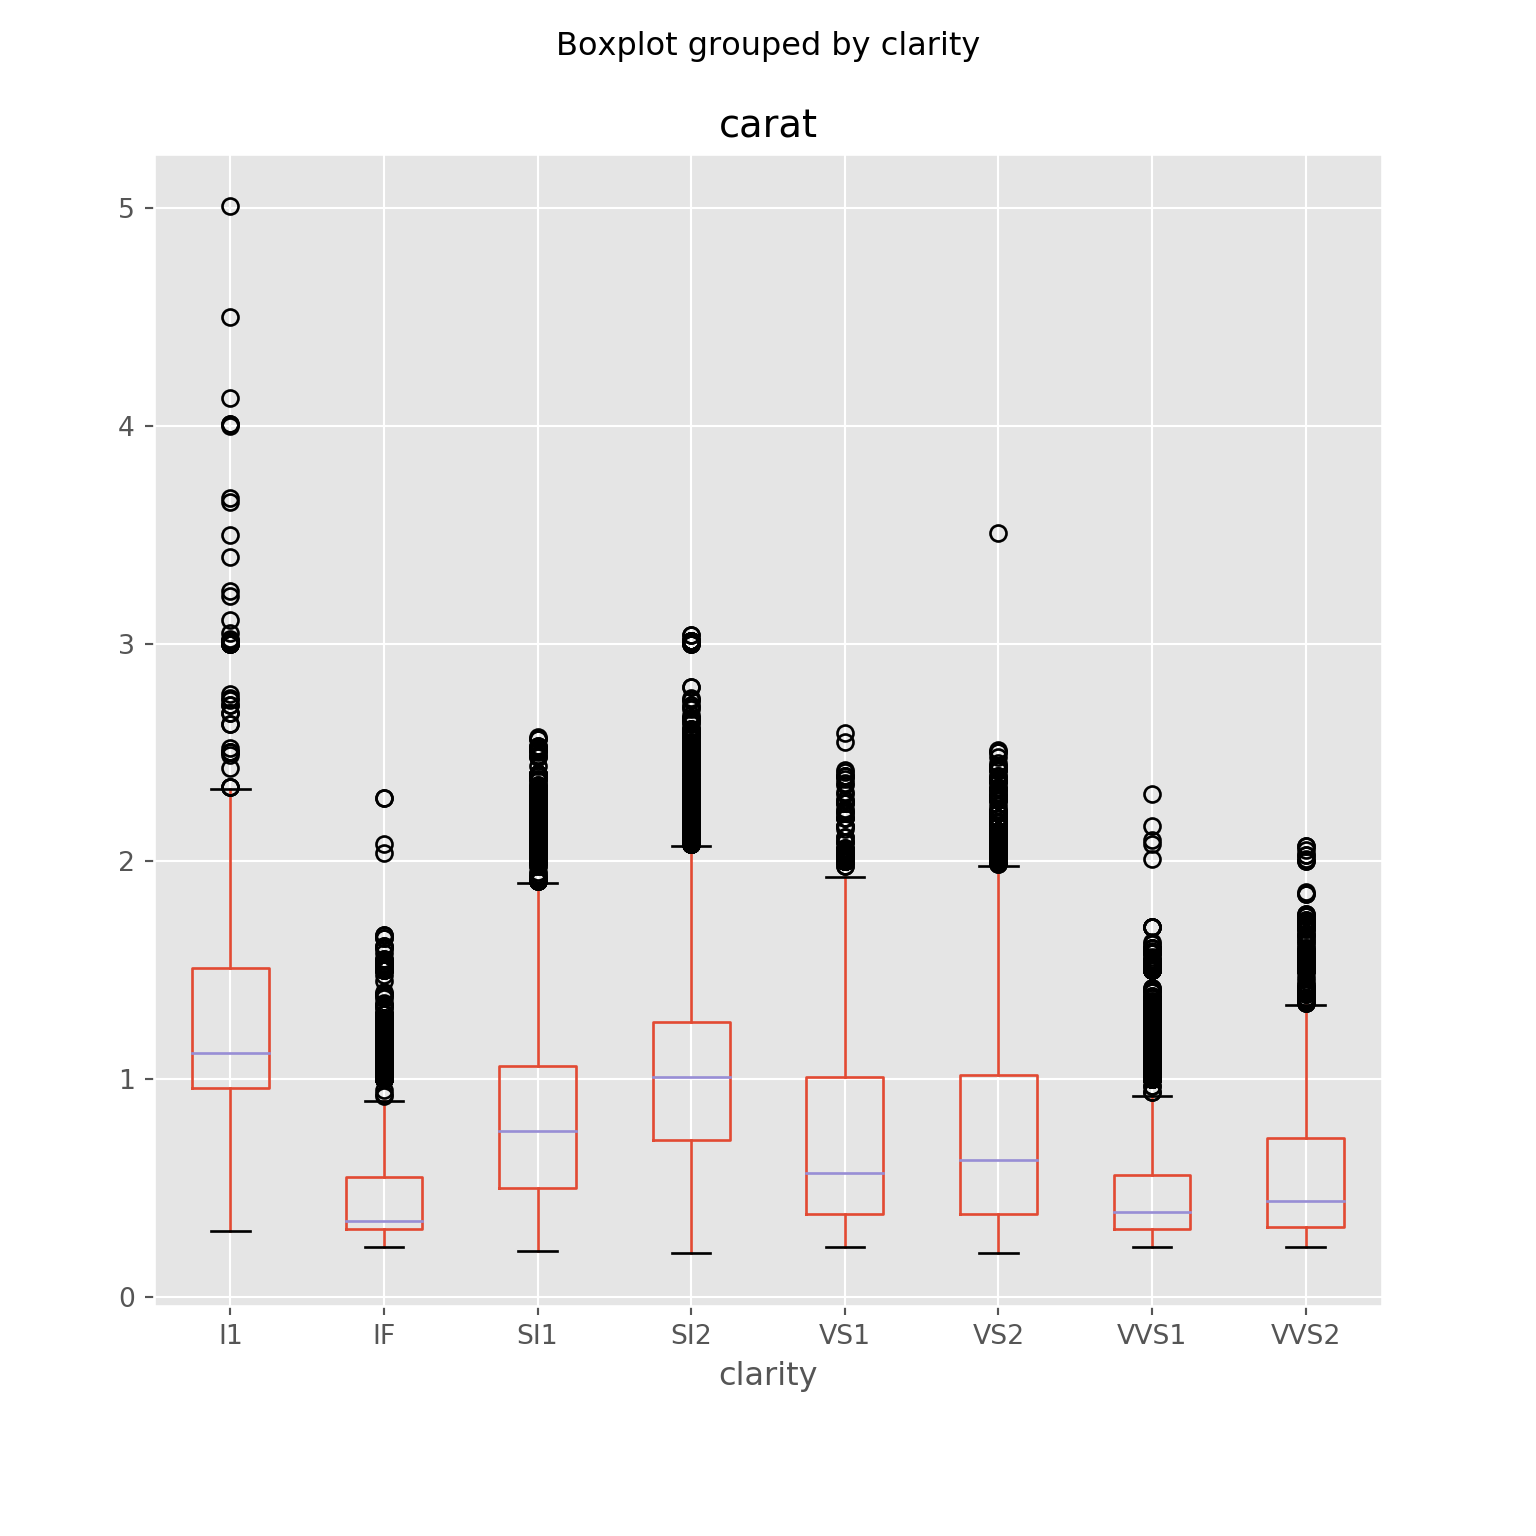
\includegraphics{1-Representación-Grafica-en-R_files/figure-latex/unnamed-chunk-6-1} \end{center}

\end{document}
